\section{Scheduler}\label{sec:Scheduler}
Only two tasks are running on the microcontroller, the control algorithm and the communication. The handling of these tasks is however critical. The Vicon system frequency sets a limit for the rate at which the control algorithms can be executed. It is also desirable for the control task to be executed periodically, and at any other time, the microcontroller should listen for new data on the network. Furthermore, the transmission and the control task are not synchronized.
\\
A scheduler can handle priorities and timing of tasks, for this purpose a real time operating system (RTOS) is used, FreeRTOS \cite{freeRtos}. The capabilities of this RTOS ranges beyond the needs in this project, but provides the necessary tools, and constitutes a flexible base with room for future development.

In \autoref{lst:scheduler} the two main tasks are created using \lstinline[style=customcppinline]{xTaskCreate()} and the task scheduler is started with \lstinline[style=customcppinline]{vTaskStartScheduler()}.
\vspace{-0.5 cm}
\begin{lstlisting}[style=customcpp,
                    caption={Code for initialization, creation of the different tasks, start sequence for the motors and call to the scheduler.}, 
                    label=lst:scheduler]
int main()
{
    ... 
  	// xTaskCreate(FunctionForTask,DebugName,AllocatedStackDepth,Parameters,Priority,TaskHandle)
    // Control Task -> Highest priority
    xTaskCreate(Controllers, "Control", 1000, NULL, configMAX_PRIORITIES - 1, NULL );
    // Communication Task 
    // xHandle is used for resetting the task if it gets preempted by the Control Task
    xTaskCreate(Communication, "Com", 1000, NULL, configMAX_PRIORITIES - 2, &xHandle);
    ...
    // Scheduler Start 
    vTaskStartScheduler();
    return 0;
}
\end{lstlisting}
\vspace{-0.5 cm}
Once the task scheduler is started the program never returns to main again. The scheduler has a configurable tick-rate, set to \SI{1}{ms}, which it uses for scheduling and timing tasks. The RTOS is set up to run with preemption, such that the higher priority task, \lstinline[style=customcppinline]{Control}, can preempt the lower priority, \lstinline[style=customcppinline]{Com}, in order to achieve a periodic execution of the control algorithms. The handle \lstinline[style=customcppinline]{xHandle} is used to resets the communication task if it is preempted while reading data. Since the XBee always sends data, whenever ready, out on the RX-pin of the microcontroller, data will be lost if the communication is preempted while data is on RX. In \autoref{fig:timingDiagram} an example of task occurrences in the microcontroller is shown. In this case, the preemption of the communication task happens at \SI{105}{ms}.

To make sure that there is always new data available for each execution of the control task, the execution frequency is chosen low enough such that at least one package is received in each period.

At \SI{35}{ms} in \autoref{fig:timingDiagram}, the data decoding is preempted by the control task. Since the data is already stored, decoding the package is continued by the scheduler after servicing the control task, and the data will be ready for use at the next control cycle.

\begin{figure}[H]
    \flushleft
    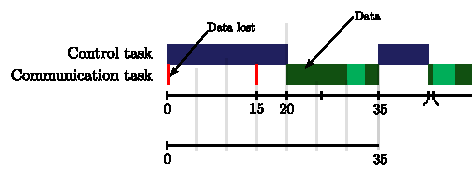
\includegraphics[width =.95\textwidth]{figures/timingDiagram}	
    \caption{An example of task execution schedule. The control task is periodic and the packages can arrive at different instances.} 
    \label{fig:timingDiagram}
\end{figure}

Although the packages are received at instances unrelated to the control task, the packages still arrive periodically, though the period may fluctuate.
\newpage